%  Bachelorarbeit                                           %%
%% TH Köln -Campus Gummersbach, Fak. 10)                    %%
%% 2021                                                     %%
\documentclass[a4paper,12pt,oneside]{article}
% Optionen:
% - a4paper => DIN A4-Format
% - 12pt    => Schriftgröße (weitere  
%              grundlegende Fontgrößen: 10pt, 11pt)
% - oneside => Einseitiger Druck

%% Verwendete Pakete:
\usepackage[ngerman]{babel} % für die deutsche Sprache
\usepackage{caption} % Für schönere Bildunterschriften
\usepackage[T1]{fontenc} % Schriftkodierung (Für Sonderzeichen u.a.)
\usepackage[utf8]{inputenc} % Für die direkte Eingabe von Umlauten im Editor u.a.
\usepackage{fancyhdr} % Für Kopf- und Fußzeilen
\usepackage{lscape} % Für Querformat

%% Show code in a better way
\usepackage{listings}
\usepackage{color}

\definecolor{dkgreen}{rgb}{0,0.6,0}
\definecolor{gray}{rgb}{0.5,0.5,0.5}
\definecolor{mauve}{rgb}{0.58,0,0.82}

\lstset{frame=tb,
  language=Java,
  aboveskip=3mm,
  belowskip=3mm,
  showstringspaces=false,
  columns=flexible,
  basicstyle={\small\ttfamily},
  numbers=none,
  numberstyle=\tiny\color{gray},
  keywordstyle=\color{blue},
  commentstyle=\color{dkgreen},
  stringstyle=\color{mauve},
  breaklines=true,
  breakatwhitespace=true,
  tabsize=3
}
%% Schriften (Beispiele)
%% Weitere LaTeX-Schriften im "LaTeX Font Catalogue"
%% unter: http://www.tug.dk/FontCatalogue/.
%% ACHTUNG: Ggf. müssen Schriften noch installiert 
%% werden!

% Serifen-Schriften:
\usepackage{lmodern} % Schriftart "Latin Modern"
%\usepackage{garamond} % Schriftart "Garamond"

%Sans Serif-Schriften:
%\usepackage[scaled]{uarial}
%\usepackage[scaled]{helvet}
%%--------------
\usepackage[normalem]{ulem} % Für das Unterstreichen von Text z.B. mit \uline{}
\usepackage[left=3cm,right=2cm,top=1.5cm,bottom=1cm,
textheight=245mm,textwidth=160mm,includeheadfoot,headsep=1cm,
footskip=1cm,headheight=14.599pt]{geometry} % Einrichtung der Seite 

\usepackage{graphicx} % Zum Laden von Graphiken
\graphicspath{ {./sources/} }

% INFO: Graphiken einbinden
%
% \includegraphics[scale=1.00]{dateiname}
%
% => Ausgabeformat: PDF-Dokument:
%    Es können die folgenden (Graphik-)formate eingebunden
%    werden: .jpg, .png, .pdf, .mps
% 
% => Ausgabeformat: DVI/PS:
%    Folgende (Graphik-)formate werden unterstützt:
%    .eps, .ps, .bmp, .pict, .pntg
\usepackage{epstopdf}

% Pakete für Tabellen
\usepackage{tabularx} % Einfache Tabellen
\usepackage{longtable} % Tabellen als Gleitobjekte (für die Aufteilung bei langen 
 %Tabellen über mehrere Seiten)
\usepackage{multirow} % Für das Verbinden von Zeilen innerhalb einer Tabelle mit
 % \multirow{anzahl}{*}{Text}

% (Zusatz-)Pakete für Formeln
\usepackage{amsmath}
\usepackage{amsthm}
\usepackage{amsfonts}

\usepackage{setspace} % Paket zum Setzen des Zeilenabstandes
% INFO: Zeilenabstand setzen:
%
% Befehle:
% - \singlespacing  => 1-zeilig (Standard)
% - \onehalfspacing => 1,5-zeilig
% - \doublespacing  => 2-zeilig 
\onehalfspacing % Zeilenabstand auf 1,5-zeilig setzen

% Farbboxen (für die Merkkästen in dieser Vorlage):
\usepackage{tcolorbox}
\tcbset{colback=white,colframe=orange,
        fonttitle=\bfseries}

\usepackage[colorlinks,pdfpagelabels,pdfstartview=FitH,
bookmarksopen=true,bookmarksnumbered=true,linkcolor=black,
plainpages=false,hypertexnames=false,citecolor=black]{hyperref} % Für Verlinkungen
% INFO: Verlinkungen mit dem hyperref-Paket:
%
% Die Angabe von URLs mit dem Befehl \url{} erlaubt einen
% gesonderten Umgang mit Weblinks. Denn die Links werden verlinkt.
% Auch erfolgt automatisch am Zeilenende ein Umbruch des Links.
% Es ist auch nicht erforderlich, Sonderzeichen in der URL manuell zu 
% entschärfen.
%
% TIPP: Sollte ein Umbuch bei einem Link nicht automatisch erfolgen, so kann
% das daran liegen, dass ein/mehrere Zeichen zusätzlich angegeben werden müssen,
% an dem der Link umbrochen werden kann.
% Dies kann mit folgendem Befehl erfolgen (Beispiel):
% \renewcommand*\UrlBreaks{\do-\do_}

% Das Paket "biblatex" für autom. 
% Literaturverzeichnisse:
%\usepackage{csquotes} % Für sprachangepasste Anführungszeichen
%\usepackage[backend=bibtex,style=alphabetic]  
%           {biblatex}
%\addbibresource{bib/literatur.bib}           

%%%%%%%%%%%%%%%%%%%%%%%%%%%%%%%%%%%%%%%%%%%%%
%% DOKUMENT                                %%
%%%%%%%%%%%%%%%%%%%%%%%%%%%%%%%%%%%%%%%%%%%%%

\begin{document}
% Unbeschriftetes Vorblatt (Leere Seite)
\pagestyle{empty} % Seite ohne Kopf- und Fußzeilen
\newpage % Neue Seite
\input{leereSeite} % Ausgelagerte LaTeX-Datei (hier: leereSeite.tex) einbinden

\newpage

% Deckblatt
\pagestyle{empty}
\begin{titlepage}
  
\includegraphics[scale=0.20]{sources/TH_Koeln_Logo}\\
  \begin{center}
    \Large
    Technische Hochschule Köln\\
    Fakultät für Informatik und Ingenieurwissenschaften\\
    \hrule\par\rule{0pt}{2cm} % Horizontale Trennlinie  mit 2 cm Abtand nach unten erzeugen
    \LARGE
    \textsc{BACHELORARBEIT}\\
    \vspace{1cm} % Vertikaler Abstand von 1cm erzeugen
    \huge
    Kostenoptimierung für Cloud-Diensten \\
    \Large
    Ein wirtschaftlicher Ansatz für Amazon Web Services\\
    \vspace{1cm}
    \large
    Vorgelegt an der TH Köln Campus Gummersbach\\
    im Studiengang Wirtshaftsinformatik\\
    \vspace{1.0cm}
    ausgearbeitet von:\\
    \textsc{Carlo Menjivar} 11117929\\
    \vspace{1cm}
    \begin{tabular}{ll} % Einfache Tabelle ohne Rahmen, mit 2 Spalten erzeugen
      \textbf{Erster Prüfer:}  & Prof. Dr. Roman Majewski \\
      \textbf{Zweiter Prüfer:} & <Name des 2. Prüfers>    \\
    \end{tabular}
    \vspace{1cm}
    \\Gummersbach, im F<Monat der Abgabe>
  \end{center}
\end{titlepage}

\newpage

% Abstract (ACHTUNG: Abweichung zur Reihenfolge im Merkblatt!)
\begin{abstract}
  Platz für das deutsche Abstract...
\end{abstract}

\renewcommand{\abstractname}{Abstract}
\begin{abstract}
  Platz für das englische Abstract...
\end{abstract}
%<MERKKASTEN> (für die eigene Verwendung bitte entfernen
\vspace{1cm}
\begin{tcolorbox}[title={Das Abstract}]
  Bei einem Abstract handelt es sich um eine Art \textit{Zusammenfassung} Ihrer Arbeit. Diese kann in deutscher und/oder englischer Sprache verfasst werden. Mithilfe des Abstracts kann der Leser sich zügig orientieren, in wie fern Ihre Arbeit für ihn Relevanz besitzt.\\                                                                      Sprechen Sie unbedingt mit Ihrer Betreuerin/Ihrem Betreuer, ob Sie für Ihre Arbeit ein Abstract benötigen.\\
  Ein Abstract beinhaltet folgende Aspekte \footnote{ Vgl. \cite{SW11}, S. 249}:
  \begin{itemize}
    \item Ziel der Arbeit
    \item Fragestellung der Arbeit
    \item Herangezogener, theoretischer Ansatz ("Quellen")
    \item \textit{Optional:} Methodik
  \end{itemize}
\end{tcolorbox}
%</MERKKASTEN>

%<MERKKASTEN> (für die eigene Verwendung bitte entfernen
\vspace{1cm}
\begin{tcolorbox}[title={Hinweise zu dieser Dokumentvorlage}]
  \begin{itemize}
    \item Es handelt sich hierbei um eine Beispiel-Vorlage für wissenschaftliche Ausarbeitungen.
          Über die konkrete, formale Ausgestaltung Ihrer wissenschaftlichen Arbeit sprechen Sie unbedingt mit Ihre/m Betreuer/in.
    \item Unabhängig, ob Sie beispielsweise eine Bachelor-, Master- oder Hausarbeit schreiben müssen. Diese Vorlage kann als eine gute Basis für Ihre Arbeit dienen. Passen Sie einfach die Vorlage Ihren Anforderungen entsprechend an.
  \end{itemize}
\end{tcolorbox}
%</MERKKASTEN>  

\newpage

% Inhaltsverzeichnis
\tableofcontents

\newpage
\pagestyle{fancy} % Kopf- und Fußzeilen aktivieren (=> Paket "fancyhdr")

% Abbildungsverzeichnis  
% INFO: Abbildung einbinden (Beispiel):
%  \begin{figure}[h!]
%    \centering
%    \includegraphics[scale=1.00]{Pfad zum Bild}\\
%    \caption{Bildunterschrift} 
%    \label{Marke zum Referenzieren auf die Abbildung}
%  \end{figure}
\section*{Abbildungsverzeichnis}
\addcontentsline{toc}{section}{Abbildungsverzeichnis} % Manuellen Eintrag im Inhaltsverzeichnis erzeugen
\renewcommand{\listfigurename}{} % Name des Abbildungsverzeichnisses ändern
\thispagestyle{empty}
\listoffigures

\newpage
% INFO: Querverweise auf Gliederungselemente, Abbildungen 
%       & Tabellen setzen:
%
% Voraussetzung: Gesetzte Referenzmarke mit dem Befehl: \label{marke}
% 
% Referenzierung erfolgt dann mittels dem Befehl:
% \ref{marke}

\section{Einleitung}\label{kap_einleitung}
%Motivation und Ziele als subsecion?
%WEITERE QUELLE Für mOTIVATION
%https://www.gartner.com/smarterwithgartner/4-trends-impacting-cloud-adoption-in-2020
%\subsection*{Einführung in das Thema (Motivation, zentrale Begriffe etc.)}
\subsection{Motivation}
%\addcontentsline{toc}{subsection}{Motivation}
%WARUM HABE ICH MICH FÜR AWS ENTSCHIEDEN?
%Wie viele Firmen wechseln von On-Premise zu Cloud in DE jährlich?
[Persönliches Statement... wieso schreib ich das hier eigentlich ;)] Die zunehmende Digitalisierung von Geschäftsmodellen, die auch durch die Corona-Pandemie vorangetrieben wird, lässt Cloud-basierte Applikationen an Bedeutung gewinnen.\footnote{Es sei an diser Stelle darauf hingewiesen, dass in diesem Kontext Ahrens die Bedeutung Cloud-basierter Anwendungen im Bereich von deutschen Handelsunternehmen untersuchte (Vgl. Ahrens 2021)\cite{STA3}, sowie das \textit{ifo Institut} anschaulich die strukturellen Veränderungen von der Corona-Pandemie auf den Arbeitsalltag in Deutschland nachzeichnete (Vgl. ifo Institut 2020)\cite{STA2}.} Als direkte Folge davon ist die Nachfrage nach Server- und Speicherkapazität gestiegen.
%Dies wird auch von 48\% der befragten Handelsunternehmen im Jahr 2021 bestätigt.
Die Relevanz von \textit{Amazon Web Services}, kurz AWS, in dem Bereich der Cloud-Computing ergibt sich aus einer vor kurzem veröffentlichte Studie von Raj Bala et al.. Diese wies eindrücklich daraufhin, dass AWS der aktuell weltweit führende Cloud-Anbieter anhand ihrer Klassifikation (\textit{Magic Quadrant}\footnote{ Laut Gartner stellt der Magic Quadrant eine zweidimensionale Matrix mit vier Quadranten dar. Jeder Quadrant steht für einen Unternehmenstypus im Markt. Im Uhrzeigersinn von links unten beginnend sind dies: \textit{Nichenanbieter, Herausforderer, Marktführer }und \textit{Visionäre}}) für Cloud-Infrastruktur und Plattform-Services sei (Bala et al, 2021, o.S.,\cite{G01}).
AWS erscheint nicht nur aus diesem Grund als Fallbeispiel für diese Arbeit passend, weitere bedeutsame Faktoren sind seine frühe Präsenz (2006) als Cloudanbieter und seines großen Angebotes an Cloud-Diensten, welche für zahlreiche Anwendungsfälle geeignet sind.\footnote{ Die aktuellen Marktführer im Bereich der \textit{Cloud-Computing} weltweit sind AWS, Google, Telekom und Microsoft (Vgl. Synergy Reseach Group 2019, o.S.\cite{STA6})}
\\\\

\begin{comment} GELÖSCHT, WEIL DIESE EINE BEHAUPTUNG IST (25.10.2021)
    \\\\
    Für viele Unternehmen ist eine große Herausforderung, die Kosten von Cloud-Diensten übersichtlich zu halten und Optimierungsmöglichkeit leicht zu erkennen. Zusätzlich besteht die Gefahr, unangenehme Überraschungen in einer Rechnung zu bekommen, weil keine Grenze für den Konsum von Cloud-Diensten festgelegt wurde. 
    \end{comment}
\subsection{Problemstellung}
%\addcontentsline{toc}{subsection}{Problemstellung}
%Wenn ein Hotel die Vorteile von dem Cloud-Computing hätte, dann könnte dieses folgendermaßen funktionieren:
\begin{comment}
\\\\
”Heute hatten wir 17 Gäste für unsere derzeit 20 Zimmer. Für die kommende Messe am Wochenende sind wir bereit 500 Gäste zu empfangen. Nach der Messe werden wir mit unseren üblichen 20 Zimmern wie immer gut arbeiten können.”
Normalerweise bräuchte man eine große Investition zu machen, um solche kurzfristige Nachfrage zu erfüllen. Vergleichbar ist es bei traditionellen IT-Infrastrukturen, mehr Kapazitätsbedarf, würde die Anschaffung von einer neuen Hardware bedeuten.
\\\\
\end{comment}
%Die Verwendung von Cloud-Diensten bringt viele Vorteile mit sich. Zum Beispiel kurzfristige Erhöhung oder Verringerung der Speicher- und Rechenkapazität, sowie Zugriff auf unterschiedliche Speicherarten, die genau an individuelle Anwendungsfälle angepasst sind. All diese Lösungen sind in wenigen Minuten einsatzfertig. 
%\\\\
%Viele Unternehmen befürchten jedoch, dass der Wechsel von On-Premise zu On-Demand zu hohen Kosten führen könnte.
%In einer Umfrage haben circa 50\% der Unternehmen die Verwaltung der Kosten für den Betrieb von Cloud-Workloads als großes Hindernis genannt. Mehr als die Hälfte der Befragten haben geäußert, dass sie Schwierigkeiten haben, alle Kosten für Cloud-Workloads zu rechtfertigen.
Adam Stern wies in dem \textit{Forbes}-Magazin daraufhin, dass ungefähr die Hälfte der US-amerikanischen Unternehmen Schwierigkeiten hätten ihre Kosten zu begründen (Stern 2018, o.S.). 
\begin{quote}
    „In its Stratecast Predictions 2018, Frost \& Sullivan noted that 53\% of IT leaders surveyed cited “managing costs to run cloud workloads” as a huge obstacle, and over 50\% have difficulty justifying the expenses of some public cloud workloads.“  
    \footnote{Stern, Adam, The Truth About Cloud Pricing.\cite{SP1}}
\end{quote}
Darüber hinaus weist Tobias Regenfuß und Jochen Malinowski
von Accenture GmbH in einer Untersuchung, dass es den Unternehmen an fachlichem Know-How in Cloud-Computing mangelte. Diese stelle eine der größten Hindernisse dar, um einen Wechsel von On-Premise- zu Cloud-basierten Systemen gewährleisten zu können\footnote{Regenfuß und MalinowskiStern, Hohe Erwartungen an die Cloud: Hürden meistern, Mehrwert maximieren. 2020 o.S.(Webversion) oder S.11 in der PDF-Version auf Englisch\cite{ACC1}}.
\\\\
Kostenoptimierung für Cloud-Dienste ist ein wichtiger Punkt, da man ohne Optimierungsmaßnahmen mit höheren Kosten rechnen müsse als bei On-Premise Systemen(Anders Lisdorf\footnote{Anders Lisdorf. Cloud Computing Basics: a Non.-Technical Introduction. S.152. \cite{CCB}}).
\\
([Rev] SOLLTE DIE UNTERE DIREKTE ZITAT WEG)
\begin{quote}
    ”Indeed, if you run the cloud the same way you run your on-premise data center, you are almost certain to incur higher expenses. It is necessary to use the following key cloud cost optimization techniques in order to successfully save money on the cloud.”
    \footnote{Anders Lisdorf. Cloud Computing Basics: a Non.-Technical Introduction. S.152. \cite{CCB}}
\end{quote}
\begin{flushleft}
Diese Bachelorarbeit beschäftigt sich mit ebendieser Problematik, um herauszufinden, wie Unternehmen mit den passenden Werkzeugen die Kosten ihrer Cloud-Dienste überwachen und im Blick behalten können. %Zum Beispiel können frühzeitige Benachrichtigungen alarmieren, wenn Cloud-Dienste mehr Kosten verursachen als geplant.
\\
Außerdem sollte untersucht werden, wie mit der richtigen Auswahl an Diensten Kosten optimiert werden. 
%In dieser Arbeit wird versucht zu beantworten, wie Kosten bei Cloud-Diensten überwacht werden können. Auf Grundlage dieser Information werden Optimierungsmöglichkeiten untersucht. 
Es wird untersucht, welche Maßnahmen nötig sind, um unerwartet hohe Kosten bei Cloud-Diensten zu vermeiden. Darüber hinaus werden Empfehlungen von Cloud-Experten berücksichtigt, um Kosten von Cloud-Diensten zu minimieren. Diese Arbeit untersucht speziell die Kostenoptimierung  von S3-Speichereinheiten und EC2-Server-Instanzen mithilfe von folgenden Überwachungswerkzeuge: Cost-Explorer, CloudWatch und Trusted Advisor.
\end{flushleft}


\subsection{Zielsetzung}
%\addcontentsline{toc}{subsection}{Zielsetzung}
Die vorliegende Arbeit betrachtet die von AWS angebotenen Überwachungswerkzeuge, um ein tiefergehendes Verständnis der Entstehung von Kosten durch die Nutzung von Cloud-Diensten zu gewährleisten. Mit den von AWS zur Verfügung gestellten Maßnahmen sollen die Nutzung und damit die Kosten von Cloud-Diensten reduziert werden.
%\textbf{Daraus ergeben sich für die Arbeit die folgenden Ziele:}%\\ 
%\%begin{itemize}
 %   \item
 %       Als Erstes wird gezeigt, wie mithilfe von bestehenden %Werkzeugen  die Kosten von Cloud-Diensten überwacht %werden können.
  %  \item
 %       Als Nächstes wird anhand von Empfehlungen von Cloud-Experten identifiziert, welche Optimierungsmöglichkeiten bestehen.\\
%\end{itemize}

%Die vorgestellten Werkzeuge werden auf eine Testumgebung eingesetzt und deren Auswirkungen im Bezug auf die Kosten %bewertet.\\
\begin{comment}
\subsection*{Einschränkungen}
\addcontentsline{toc}{subsection}{Einschränkungen}

Der Schwerpunkt dieser Arbeit liegt auf EC2-Instanzen, da diese in der Regel den größten Anteil an der Rechnung ausmachen.
An zweiter Stelle stehen S3-Speichereinheiten, weil sie einen erheblichen Teil der Kosten darstellen.
%STATISTEN DIE DAS BELEGEN?

%Nach Angaben von Amazon Web Services ist es möglich bis zu 90% für EC2 zu sparen, wenn EC2 Spot-Instanzen benutzt werden. 
%Eine Preisreduzierung für Speichereinheiten ist möglich, wenn die richtige Speicherart ausgewählt wird. 
{\cite{AMZ08,AMZ09}} 
\\
Diese Arbeit legt den Fokus auf die Optimierung der oben genannten Dienste.
Als Überwachungswerkzeuge für die Kosten werden die AWS CloudWatch, der AWS Cost-Explorer und der AWS Trusted Advisor untersucht. 
\end{comment}
\subsection{Struktur der Arbeit}
%\addcontentsline{toc}{subsection}{Struktur der Arbeit}

%Schlüsselbegriffe
%Zunächst wird es eine kurze Einführung in die relevanten Begriffe geben, die für die zu untersuchenden AWS-Cloud-Services wichtig sind.

Diese Bachelorarbeit ist in folgende Kapitel unterteilt:\\\\
%2 Die gängigsten Cloud-Dienste, bei deren Geld verschwendet wird.
\textbf{Kapitel~\ref{kap_grundlagen}} 
befasst sich mit dem Begriff Cloud-Economy und erläutert das Potenzial der Cloud-Diensten im wirtschaftlichen Sinne. Die Cloud-Dienste EC2-Instanzen und S3 Speichereinheiten werden ebenfalls kurz erklärt. %Diese dienen als Grundlage für diese Arbeit. 
\\\\
%4 Überwachung von Kosten
\textbf{Kapitel~\ref{kap_zahlungsmodelle}} 
zeigt die verschiedenen Zahlungsmodelle für EC2-Instanzen. Es werden Kriterien vorgestellt, die helfen sollen, sich für das richtige Zahlungsmodell bei verschiedenen Szenarien zu entscheiden. 
\\\\
%5 AWS Cost Explorer und AWS-Kosten- und Nutzungsbericht
\textbf{In Kapitel~\ref{kap_kostenüberwachung }} werden die Werkzeuge eingeführt, die zur Überwachung der Kosten von Cloud-Diensten eingesetzt werden.
\\\\
%4 Methoden zur Kostenbremse
%4.1 S3 Intelligent-Tiering
%4.2 Instance-Scheduler für EC2 und AWS Reserved-Instance
\textbf{Kapitel~\ref{kap_Optimierung}} befasst sich mit Optimierungsmaßnahmen %insbesondere 
für EC2-Instanzen und S3 Speichereinheiten.

%Testumgebung
%Schließlich werden anhand eines Fallbeispiels in \textbf{Kapitel 5?}, die oben genannten Werkzeuge und Techniken in einer %kostenlosen Testumgebung getestet. Um die Zuverlässigkeit der Ergebnisse zu gewährleisten, wird alles gemacht, um die %Vorher- und Nachher-Szenarien vergleichbar zu machen. Dabei werden die Anzahl der Instanzen und deren Auslastung sowie %die Daten auf den Speichereinheiten berücksichtigt.
 

\newpage

\section{Grundlagen}\label{kap_grundlagen}
In diesem Grundlagenkapitel werden Erfolgschancen für Unternehmen aufgelistet, die Cloud-Dienste in ihre Geschäftsprozesse integrieren. Mit Cloud-Diensten sind die Dienste eines beliebigen Cloud-Anbieters im Allgemeinen gemeint und nicht ausschließlich AWS-Dienste. 
Es wird ebenfalls erklärt warum Kostenoptimierung und -überwachung relevant für Unternehmen sind.
\\\\
Folgende Ergebnisse könnten durch die Einführung von Überwachungs- und Optimierungsmaßnahmen erreicht werden:
\begin{itemize}
      \item
            Die Möglichkeit, die Kosten verschiedener Projekte, die über dieselbe Infrastruktur laufen, zu trennen.
            Auf diese Weise kann zwischen Projekten, die mehr, und Projekten, die weniger Kosten verursachen unterschieden werden.%Davor Kunden und nicht Projekte
      \item
            Eine beachtliche Erhöhung der finanziellen Rentabilität im Unternehmen.%[ZITAT].
      \item
            Eine geringere Ungewissheit bei der Umsetzung von cloudbasierten Systemen.
      \item
            Mehr Kontrolle über die Gesamtkosten des Betriebs, den sogenannten \textit{TCO}.\footnote{TCO steht für \textit{Total Cost of Ownership}(Vgl. Gartner, o.J., o.S.\cite{TCO}.)}{ }\footnote{Vgl. Ubuntu, delivered by Canonical: A business guide to hybrid/multi-cloud, S.2.\cite{CAN01}}

\end{itemize}
%Basandose en "Vor- und Nachteile der Nutzung von Cloud-Diensten (mit mobilen Endgeräten) in Organisationen und deren Einfluss auf die Nachhaltigkeit"
% Debería aclarar los aspectos principales de mi BA
% En mi caso: 

%1-Cuales son los miedos, razones y oportunidades para las empresas en la NUBE?

%\subsection{Risiken und Oportunitäten der Cloud...}\label{subsec_UabsGrund2}
%Vor- und Nachteile / ?

\subsection{Cloud Economics}\label{subsec_UabsGrund3}
%Was bietet die Cloud den Unternehmen?
%Economics of Cloud Computing
%https://d1.awsstatic.com/whitepapers/introduction-to-aws-cloud-economics-final.pdf
%[Date last review: 25.11 Isa]
%\begin{flushleft}
%\textit{On-Demand Prinzip} kann zum Beispiel die Rechenkapazität je nach Bedarf angepasst werden 
\textit{Cloud Economics} befasst sich mit den Kosten und den Vorteilen von Cloud Computing und die dahinterstehenden wirtschaftlichen Grundsätzen. Anhand des \textit{Pay-as-you-go-Modell (PAYG)} können zum Beispiel nur die Cloud-Dienste in Anspruch genommen werden, die in dem Moment für das Unternehmen gebraucht werden. Damit entfällt die Notwendigkeit hohe Investitionen in Hardware zu tätigen, wie bei On-Premise-Systemen, wo Hardware im Voraus für den künftigen Bedarf.\footnote{Vgl. Anders Lisdorf, 2021, Cloud Computing Basics: a Non.-Technical Introduction, S.23\cite{CCB}} Durch den Verzicht auf Hardware entfallen die Kosten für Reparatur und Wartung. Die Cloud-Anbieter übernehmen dabei viele Verwaltungsaufgaben. Laut Larry Carvalho und Matthew Marden führe dies zu einer Abnahme der nötigen Fachkräften.\footnote{Larry Carvalho and Matthew Marden, 2015, Quantifying the Business Value of Amazon Web Services, S.1\cite{IDC01}} So ist die die Nutzung von Cloud-Diensten in unabhängiger Weise möglich; in Selbstbedienung und mit der Freiheit Dienste ohne Einschränkungen zu gebrauchen. Das bedeutet jedoch gleichzeitig, dass die Nutzerin oder der Nutzer von Cloud-Diensten Verantwortung für die anfallenden Kosten übernehmen.
%\end{flushleft}
%[Grafik der Kosten On-Premise/Demand?]

\subsubsection{Skalierbarkeit}
Hierbei bezieht sich diese Arbeit auf die Möglichkeit, die Kapazität von Cloud-Diensten zu skalieren. Um die Leistung der IT-Infrastruktur aufrecht zu halten, ist es zum Beispiel möglich, das Serversystem so zu konfigurieren, dass es auf wechselnde Lastanforderungen reagiert.
%bietet  ist es möglich die Rechenkapazität hoch- und runterzuskalieren.
%Vertikal und Horizontal
%
%DOPPELT?Mit Auto Scaling wird sichergestellt, dass die Rechenkapazität in Zeiträumen von hoher Nachfrage automatisch hochskaliert.[AUCH RUNTER?]
% davor:  Anzahl der Amazon Server-Instanzen ABER ANZAHL VON SERVERN != Rechenkap.
% und damit Kosten minimieren.
Auf diese Weise kann Zeit mit der Verwaltung von IT-Infrastruktur eingespart werden, welche dann genutzt werden kann, um sich auf die wesentlichen Geschäftsaktivitäten zu konzentrieren.
\footnote{Mark Wilkins, 2021, AWS Certified Solutions Architect - Associate (SAA-C02), S.29.\cite{AWS1}}
%\parencite[][Seite 29]{AWS1} 
%\footnote{Vgl. [p.~29]\cite{AWS1}[]}
%OPTION 2: 
%Auf diese Weise wird Zeit mit der Verwaltung von IT-Ressourcen gespart und es kann sich auf die wesentlichen Geschäftsaktivitäten konzentrieren.
% Davor: 
%Auf diese Weise kann weniger Zeit mit der Verwaltung von IT-Ressourcen verbracht werden und sich mehr auf wesentliche Geschäftsaktivitäten konzentriert werden\footnote{Vgl. {\cite{AWS1}}, Seite 29}.
%\\\\
Dies war der Fall bei \textit{Walgreens} im Jahre 2020 in den Vereinigten Staaten.
Sie haben unter anderem 750 virtuelle Maschinen und \textit{SAP HANA} auf \textit{Azure Instanzen} migriert.
Diesbezüglich kommentierte Dan Regalado:
\begin{quote}
      By getting out of the business of managing datacenters, WBA[Walgreens Boots Alliance] can spend less time worrying about managing IT resources and more time focusing on what it’s really good at—delivering great healthcare and retail experiences to its customers. Azure also gives WBA an opportunity to better utilize the capabilities of its SAP implementation. “One of the key reasons for moving to Azure was so that we could take advantage of the scalability that SAP HANA is capable of,” explains Regalado. “Instead of using extremely big SAP HANA Large Instances, we can start using smaller VMs[virtuelle Maschinen] and then scale out.\footnote{Microsoft, 2020, Customer Story-Walgreens Boots Alliance delivers superior customer service with SAP solutions on Azure, o.S. \cite{AZU01}}
\end{quote}
So erklärte Dan Regalado, dass \textit{Walgreens} mit dem Einsatz von kleinen Instanzen und Auto-Scaling eine Serverinfrastruktur erreicht hat, die sich dem Bedarf an Rechenkapazität anpasst. 

\subsubsection{Flexibilität}% und Agilität}
Hiermit ist die Möglichkeit gemeint, wenn nötig und unter den Bedingungen des Cloud-Anbieters, Cloud-Dienste in Auftrag zu geben und kündigen. Für Cloud-Dienste gibt es im Allgemeinen eine Vielzahl von Optionen, von denen einige Beispiele unten aufgeführt werden:
\begin{itemize}
\item
    Verschiedene Betriebssysteme, ohne oder mit Lizenzierung.
\item
    Die meistverbreiteten Programmiersprachen, unter anderem \textit{Java, C++, Go, JavaScript und Python}.{\cite{AMZ03}}
\item
    Hosting für statische Webseiten und Webanwendungen{\cite{AMZ04}}.
\item
    Populäre relationale und nicht relationale Datenbanken{\cite{AMZ10}}.           
\item
    Vielfältige Hardware-Konfigurationen.

\end{itemize}
Durch die Vielzahl der verfügbaren Diensten ist es möglich, Prototypen und Experimente in kurzer Zeit durchzuführen.\footnote{Vgl. IDC, 2015, Business Value of AWS S.7\cite{IDC01}} Softwareprojekte können schnell auf den Markt gebracht werden. Je nach ihrem Erfolg ist es möglich, sinnvolle und kosteneffizientere Entscheidungen zu treffen. Wenn ein Projekt, aus welchen Gründen auch immer, kurzfristig eingestellt werden muss, könnten alle damit verbundenen Kosten ausfallen. Denn im Gegensatz zu On-Premise-Infrastrukturen gibt es keine Bindung an kostspielige Hardware.
%Wenn die Neuentwicklung nicht erfolgreich war, müssen keine weitere Kosten anfallen.
%Da die verwendete Dienste vollständig stillgelegt werden können.

\subsubsection{Selbstbedienung}
Mit geringem Aufwand ist es möglich, Cloud-Dienste eigenständig einzurichten. Dies hat den Vorteil, dass keine weiteren Personen, wie externe Spezialisten oder die Vertriebsabteilung des Cloud-Anbieters  benötigt werden.\footnote{Vgl. Anders Lisdorf, 2021, Cloud Computing Basics: a Non.-Technical Introduction, S.28\cite{CCB}}
Andererseits besteht ebenso die Gefahr, dass hohe ungewollte Kosten entstehen, wenn jemand versehentlich oder in unverantwortlicher Weise Dienstleistungen in Anspruch nimmt.    
%[TODO: ADD USE CASE WHERE THIS HAPPEND]
%LinkedIn Learning, the woman said something like that?
%BRINGT DIESE UNTERKAP. ETWAS ZUR ARBEIT BEI?

\subsubsection{Keine Vorabkosten}
%https://aws.amazon.com/de/ec2/pricing/
Das Pay-as-you-go-Modell (PAYG) wird von einer Reihe von Cloud-Anbietern angeboten.\footnote{Die aktuellen Marktführer im Bereich der \textit{Cloud-Computing} weltweit sind AWS, Google, Telekom und Microsoft (Vgl. Synergy Reseach Group 2019, o.S.\cite{STA6}).} Dieses erfordert keine Vorauszahlungen für die Nutzung den verschiedenen Cloud-Diensten. Wenn nur für die monatlich verbrauchten Diensten bezahlt wird, verringert sich zudem die Anfangsinvestition in die IT-Infrastruktur oder fällt ganz weg. Dies ist besonders für kleine Unternehmen bedeutsam, die nicht über die finanziellen Mittel verfügen, um in eine IT-Infrastruktur zu investieren. Es besteht jedoch die Möglichkeit, bestimmte Beträge für die zu konsumierende Dienste im Voraus zu bezahlen.\footnote{Im Unterkapitel \ref{sssec:Vorauszahlung} wird eine Berechnung der Einsparungen durch die teilweise oder vollständige Vorauszahlung der Kosten für die Nutzung von Serverinstanzen gezeigt.}  

%\subsubsection{Verfügbarkeit?} t.ly/bV1z
\subsubsection{Technische Fachkompetenz}
Bei einem Einsatz von Cloud-Diensten ist zu bedenken, dass weitere Investitionen wie technische Schulungen für das Personal erforderlich werden. Der \textit{TÜV Rheinland} bietet zum Beispiel Kurse zur Ausbildung von \textit{Cloud Architekten} an. Die Kurse dauern i.d.R. drei Tage und kosten 2.136,05 € pro Teilnehmer. Maßnahmen wie die genannten Kurse wirken so einem der Hauptprobleme entgegen, mit denen Unternehmen bei der Migration in die Cloud konfrontiert werden. Regenfuß und Malinowski stellten heraus, dass in einer von \textit{Accenture} im Jahr 2020 durchgeführten Umfrage 38\% der Befragten angaben, dass fehlende Kompetenzen im Unternehmen in Bezug auf die Cloud ein Hindernis für eine Cloud-Migration seien.\footnote{Regenfuß und Malinowski (Accenture), 2020, Hohe Erwartungen an die Cloud: Hürden meistern, Mehrwert maximieren, S.11\cite{ACC1}}
%[KOSTEN EINER IT-INFRA = SERVER+Rack]
% QUE PORTENTAJE DE LA INVERSION REPRESENTA LA INFRAESTRUCTURA DE IT EN UNA START UP Y EN UNA CORPORACION? RAZONES USAR LA NUBE(Statista)?

\subsection{Amazon Cloud-Dienste}%Sarah 6.12
Im Folgenden liegt der Fokus auf \textit{AWS-Diensten}. Einer der am häufigsten genutzten AWS-Dienste ist \textit{Amazon Elastic Computing Instances EC2}, mit dem virtuelle Maschinen erstellt werden können.\footnote{Kimberly Mlitz, 2021, Cloud infrastructure services vendor market share worldwide from 4th quarter 2017 to 3rd quarter 2021, o.S.\cite{STA4}} Ein weiterer wichtiger AWS-Dienst ist \textit{Amazon Simple Storage Service (S3)}, der zum Speichern von Objekten verwendet wird.\footnote{Objekte sind in AWS die Grundeinheit in welchen Dateien in den Amazon S3-Speichereinheiten gespeichert werden. Neben den Objekten werden Metadaten, wie das Datum der Objekterstellung und das Datum der letzten Aktualisierung gespeichert.(Vgl. Amazon Simple Storage Service User Guide, S.4\cite{AMZ18})}{ }\footnote{Amazon Elastic Computing Instances EC2 werden im Folgenden als \textit{EC2-Instanzen} und Amazon Simple Storage Service als \textit{Amazon S3} oder \textit{Amazon S3-Speichereinheiten} bezeichnet.}
\\\\
Wie Lynn Langit, eine erfahrene Cloud-Architektin, feststellte, könne bis zu 80\% der AWS-Rechnung aus Gebühren für EC2-Instanzen bestehen.\footnote{Lynn Langit, 2021, LinkedIn Learning: AWS Controlling Cost. Minute 0:20-0:45\cite{LINK2}} Laut des \textit{AWS Solutions Architekten} Daniel Peña Silva ist Amazon S3 einer der am häufigsten genutzten AWS-Dienste.\footnote{Vgl. Daniel Peña Silva, 2021, LinkedIn: Listado de todos los Servicios de AWS.\cite{LINK1}} Deshalb fokussiert sich diese Arbeit auf die Überwachungs- und Optimierungsmaßnahmen, hauptsächlich für EC2-Instanzen und Amazon S3.  %\subsubsection*{Amazon Elastic Computing Instances EC2}
%, Sektion 2 Control Costs by Service, Video AWS service type Minute 00:30}.%\subsubsection*{Amazon Simple Storage Service S3} Warum S3 t.ly/iWn3
%S3 ist der Speicherdienst für Objekte bei AWS. 
%der Rangliste vieler Informatikwebseiten und 
%BESSER: S3 WIRD IN BÜCHER WIE t.ly/IJc1 GENANNT? THIS IS A SPANISH CITAT!
\\\\
Wie aus der \autoref{fig:moreCloudStorageThanLocal} hervorgeht ist, werden darüber hinaus seit 2020 weltweit mehr Daten in Serverfarmen als auf lokalen Geräten gespeichert.\footnote{Vgl. Statista: 2020 überholt die Cloud lokale Speichermedien.\cite{STA1}} Dies bietet einerseits  Vorteile im Bezug auf die Geschwindigkeit der Arbeitsabläufe, andererseits birgt aber auch Risiken wie Datendiebstahl. Das Thema Datendiebstahl wird in dieser Arbeit nicht behandelt.%; da es den Rahmen der Untersuchung sprengen würde.
\begin{figure}[h!]
      \centering
      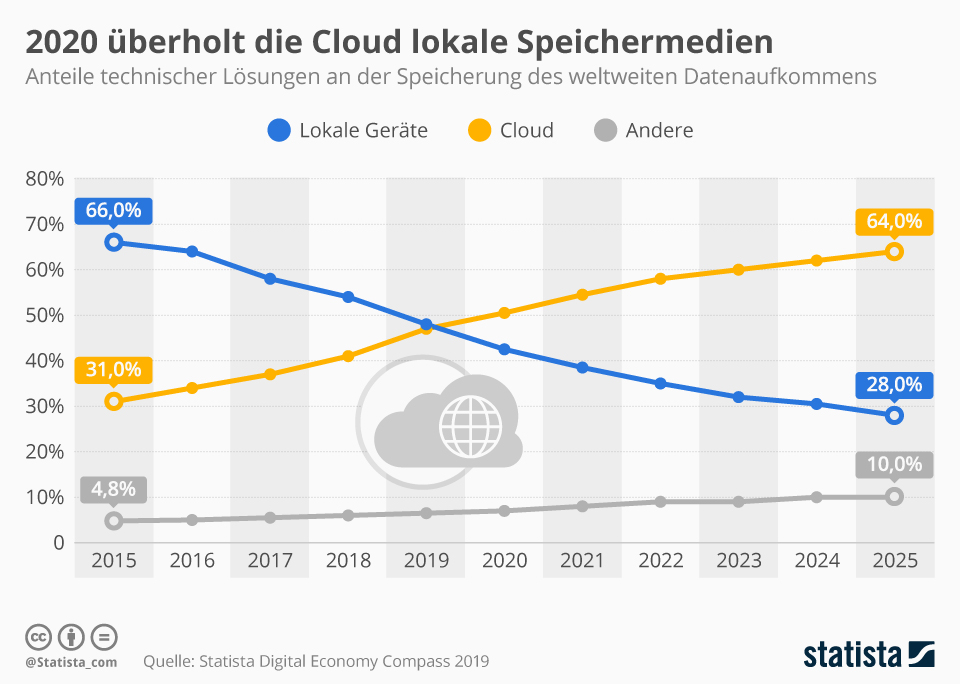
\includegraphics[scale=0.4]{sources/moreCloudStorageThanLocal}
      \caption[2020 überholt die Cloud lokale Speichermedien]{}\label{fig:moreCloudStorageThanLocal}
      2020 überholt die Cloud lokale Speichermedien, Statista, 2019 {\cite{STA1}}
\end{figure}
\\\\
\\\\
\\\\
Dieses grundlegende Kapitel hat einige potenzielle Vorteile der Nutzung von Cloud-Diensten für Unternehmen aufgezeigt. Darüber hinaus geht der Trend in den letzten Jahren zur Nutzung von Cloud-basierten Diensten. Das nächste Kapitel befasst sich mit den Zahlungsmodellen für EC2-Instanzen und den damit einhergehenden Abwägungen, die bei der Wahl dieser Modelle in verschiedenen Szenarien zu berücksichtigen sind.
\newpage

\begin{comment}
Advantages of Cloud Technology
As the technology has matured over the last decade, companies are moving to the
cloud to lower costs, reduce complexity, and increase flexibility. The cloud
provides scalable and powerful compute solutions, low-cost, reliable storage, and addition, cloud technologies can be used to deploy solutions quickly and cost effectively around the world and on any device.
When you decouple from the data center, you’ll be able to:
x Decrease your TCO: Eliminate many of the costs related to building and
maintaining a data center or colocation deployment. Pay for only the
resources you consume.

x Reduce complexity: Reduce the need to manage infrastructure,
investigate licensing issues, or divert resources.
x Adjust capacity on the fly: Add or reduce resources, depending on
seasonal business needs, using infrastructure that is secure, reliable, and
broadly accessible.
x Reduce time to market: Design and develop new IT projects faster.
x Deploy quickly, even worldwide: Deploy applications across multiple
geographic areas.
x Increase efficiencies: Use automation to reduce or eliminate IT
management activities that waste time and resources.
x Innovate more: Spin up a new server and try out an idea. Each project
moves through the funnel more quickly because the cloud makes it faster
(and cheaper) to deploy, test, and launch new products and services.
x Spend your resources strategically: Switch to a DevOps model to free
your IT staff from operations and maintenance that can be handled by the
cloud services provider.
x Enhance security: Spend less time conducting security reviews on
infrastructure. Mature cloud providers have teams of people who focus on
security, offering best practices to ensure you’re compliant, no matter what
your industry.
\end{comment}

%\subsection{Was ist EC2? To Review}\label{subsec_UabsGrund4}
%Man kann HW und SW auswählen


% Amazon video Cloud Eco.: https://www.youtube.com/watch?v=kUNBx1MTwxw
% short explaniation https://www.youtube.com/watch?v=RI9RTbXEjLc
%3- Hard and Soft Savings https://youtu.be/Q5wSvUVPyYY?t=316
% Suche ein Buch, mit info darüber!




\vspace{1cm}
\begin{tcolorbox}[title={Das Kapitel/der Abschnitt}]
  Hierbei handelt es sich um ein Beispiel-Kapitel. Es ist zu empfehlen, dass Sie Kapitel und auch Abschnitte immer mit einer kurzen Einleitung beginnen. In dieser beschreiben Sie kurz, was den Leser in diesem Kapitel/Abschnitt erwartet. Bei einem Kapitel mit Abschnitten nehmen Sie auch inhaltlichen Bezug auf die enthaltenen Abschnitte (inklusive Referenzierung auf die Abschnittsnummerierung).
\end{tcolorbox}
%</MERKKASTEN>  

\vspace{1cm}
\begin{tcolorbox}[title={Abbildungen, Tabellen \& Co.}]
  Bei Verwendung von Tabellen und auch Abbildungen beachten Sie bitte, dass diese immer Unter-/Überschriften enthalten (inklusive einer Nummer). Im Textfluss erklären/beschreiben Sie die Abbildung bzw. die Tabelle und nehmen Bezug über einen Verweis auf die Nummer.
\end{tcolorbox}


%Eizelne Kapitel
\newpage
\section{Cloud-Dienste, bei deren Geld verschwendet wird}\label{kap_DiensteGeldFresser}
% Wie werden die Informationen die Benutzer gezeigt und wie können sie diese manipulieren
\paragraph{}

\subsection{T1}


\textbf{Große Entwickler-Community}\\
\footnote{ Vgl. \cite{SO01}}
\newpage

\subsubsection{t1.2}
Bei der Auswahl des Frameworks wollten wir so unvoreingenommen wie möglich sein, daher listen wir einige Aspekte auf, die bei Projekten mit React zu beachten sind.
\newline

\textbf{Eine zu leichte Dokumentation}\\
Aufgrund der rasanten Entwicklung ist die Dokumentation in Bezug auf die neuesten Aktualisierungen und Änderungen oft spärlich. 
\footnote{ Vgl. \cite{R01}}

\subsection{T2}
\paragraph{}



\newpage
\section{Überwachung von Kosten}\label{kap_ueberwachungVonKosten }
\input{chapters/Überwachung von Kosten}
\newpage

%Temporär, danach sollten wir das Package glossaries benutzen
\section{Glossar}\label{kap_glossar}
%\newglossaryentry{kiln}
%{
 % name=kiln,
  %description={German: Brennofen (m.);\\Français: fourneau (m.)},
  %plural=kilns
%}

%Make Glossary properly...
%\acrodef{VB}{Visula Basic}

\textbf{Cloud-Computing:}\\
...
\\\\
\textbf{Cloud-Dienste:}\\
...
\\\\
\textbf{On-Demand:}\\
...
\\\\
\textbf{On-Premise:}\\
...
\\\\
\textbf{Region:}\\
Die Region ist ein völlig unabhängiges und eigenständiges geografisches Gebiet. Jede Region hat mehrere, physisch getrennte und isolierte Standorte, die als Availability Zones bekannt sind. Beispiele für Regionen sind London, Dublin, Sydney, usw \footnote{\cite{AWS1}, Seite 42}.
\\\\
\textbf{Availability Zone:}\\
Eine Verfügbarkeitszone ist einfach ein Datenzentrum oder eine Sammlung von Datenzentren. Jede Verfügbarkeitszone in einer Region verfügt über eine separate Stromversorgung, Netzwerk und Konnektivität, um die Gefahr eines gleichzeitigen Ausfalls in beiden Zonen zu verringern \footnote{\cite{AWS1}, Seite 42}.
\\\\

\textbf{Instance family:}\\
Instanzfamilien sind eine Sammlung von EC2-Instanzen, die nach dem Verhältnis von Speicher, Netzwerkleistung, CPU-Größe und Speicherwerten zueinander gruppiert sind. Zum Beispiel bietet die m4-Familie von EC2 eine ausbalancierte Kombination von Rechen-, Speicher- und Netzwerkressourcen. \footnote{\cite{AWS1}, Seite 95}.
\\\\
Instagram-Story
\\\\
Tag
\\\\
Buckets
\\\\
PAYG %https://www.nimbix.net/glossary/pay-go
\\\\
Metadaten
\\\\
Startkonfiguration %https://docs.aws.amazon.com/autoscaling/ec2/userguide/create-launch-template.html
\\\\
Scale-In/Out
%\\\\
%Governance, Compliance ?
%\\\\
\newpage

\section{Zusammenfassung und Ausblick}\label{kap_zusammfAusbl}
(To-Do:)
\\Kapitelweise Kurzdarstellung der Inhalte (inklusive Referenzierung auf die \\Kapitelnummerierung) => Nach dem Motto: \textit{Was wurde wo beschrieben?}
\\Kurzdarstellung \textit{Problem – Lösungsweg – Ergebnisse}
\\Rückkopplung auf die Einleitung: Wurde die Zielstellung der Arbeit und die \\Fragestellung zufriedenstellend beantwortet?
\\Kritische Bewertung (sofern nicht bereits im Hauptteil geschehen)
\\Offene Probleme
\\Richtung der zukünftigen/möglichen Arbeiten
\\Erläuterung, warum welche Aspekte in der Arbeit nicht erläutert 

\subsection{Umweltbezogene Aspekte}
Esta tesis habla sobre monitoreo y optimizacion de recursos de manera financiera. Pero esas dos areas enfocadas a la economia, tiene impacto en el medio ambiente por las emisiones generadas por las granjas de servidores. 
Estadisticas dicen que en Europa/Alemania se generan x toneladas de CO2 provenientes de centros de computo. Por tanto al monitoreat y reducir cosotos, se estan evitando despilfarros y al final tambien emisiones de CO2. 
\\
\subsection{Test von den Werkzeugen und Maßnahmen}
Da es in dieser Arbeit zeitlich nicht gelungen ist, die Überwachungswerkzeuge und Optimierungsmaßnahmen umzusetzen, bleibt es noch sie in einer echten Umgebung zu testen. Es wäre möglich zu verifizieren, ob die hier genannten Maßnahmen zur vergleichbaren Einsparungen führen, wie die vom Cloud-Anbieter Amazon genannten.

Amazon bietet ein kostenloses Kontingent an, die jedoch für diese Tests nicht genug war. 
\\
\subsection{Bewusstsein in der gesamten Organisation}
Zusätzlich zu den bisher genannten Maßnahmen ist es wichtig, dass Verbraucher von Cloud-Diensten Bewusstsein für die Entstehung von Kosten entwikclen.[ODER sensibilisier werden?] Von dem Entwickler bis zum der IT-Manager, jeder sollte wissen, dass es so einfach ist, Cloud-Dienste mit ein paar Klicks zu beauftragen. Diese können in kurzer Zeit ungewünschte  Kosten verursachen oder sogar über Jahre hinweg wirtschaftliche Schäden verursachen. 
%Wer wird benachrichtigt. Welche Tools? https://docs.aws.amazon.com/de_de/AWSEC2/latest/UserGuide/monitoring_ec2.html
\\
\subsection{Die richtige Personen(Owneship verbreiten)}
Die technischen Maßnahmen zur Überwachung und Kostenreduzierung wurden dargelegt, aber jemand muss diese Analysen, Anpassungen und Entscheidungen durchführen. 
Deshalb ist es wichtig, bestimmte Personen zu berücksichtigen, die die Verantwortung für das Geschehen in den Cloud-Systemen übernehmen. Idealerweise Menschen, die sich für das Thema interessieren und über die notwendigen Kenntnisse verfügen, um die gesetzten Ziele zu erreichen. 
%Sie redete über DIESES t.ly/XJ24
\\
\subsection{5G is comming}
Mit 5G ist pronostiziert, dass mehr Daten[WIE VIELE AN WELCHEM JAHR?] automatisch von Maschinen produziert werden.
\\
\subsection{Langfristige Einsparungen sollten größer als Investitionen für Optimierung sein}
Kostenoptimierung UND -Überwachung SOLLEN DIE Einsparungen NICHT ÜBERSCHREITEN . 
TRUSTED ADVISOR NICHT FÜR JEDE FIRMA.
%https://content.aws.training/video/cmcfrm/de/x2/1.0.0/jwplayer.html?endpoint=https%3a%2f%2flrs.aws.training%2fTCAPI%2f&auth=Basic%20OjUzYmEwYTZmLTk0ZmMtNDAwZi1hODBlLWQ1YzA5NmNkOWY1MA%3d%3d&actor=%7b%22objectType%22%3a%22Agent%22%2c%22name%22%3a%5b%22zEjHPzGX10miDWp26Y_cLg2%22%5d%2c%22mbox%22%3a%5b%22mailto%3alms-user-zEjHPzGX10miDWp26Y_cLg2%40amazon.com%22%5d%7d&registration=2f22bc75-44b9-4175-a976-5ba4d7fe2902&activity_id=http%3a%2f%2fid.tincanapi.com%2factivity%2ftincan-prototypes%2fgolf-example&grouping=http%3a%2f%2fid.tincanapi.com%2factivity%2ftincan-prototypes%2fgolf-example&content_token=2554ffa1-5a1e-4737-9a0f-fc3abda1083e&content_endpoint=https%3a%2f%2flrs.aws.training%2fTCAPI%2fcontent%2f&externalRegistration=CompletionThresholdPercent%7c80!InstanceId%7c0!PackageId%7ccmcfrm_de_x2_1.0.0!RegistrationTimestampTicks%7c16324112989178350!SaveCompletion%7c1!TranscriptId%7cl4fipkeHAkKh-aGlnjYdug2!UserId%7czEjHPzGX10miDWp26Y_cLg2&externalConfiguration=&width=1366&height=728&left=0&top=0
%2:25
\begin{comment}
Von Buch "Gestaltung"
  Schluss (Fazit)
Den Abschluss der Arbeit bildet die Zusammenfassung der wesentlichen
Ergebnisse, die folgende drei Punkte beinhaltet:
Beantwortung der Forschungsfrage, die Sie in der Einleitung
aufgeworfen haben.
Sinnstiftung der Arbeit: Für welchen Zweck sollen die Ergebnisse
verwendet werden?
Gegebenenfalls auch persönliche Bemerkungen und Bewertungen oder
ein kurzer Ausblick.
\end{tcolorbox}

\end{comment}

%FAZIT ist (Von Schribe)
%Was ist? Hier sollten die neue Erkenntnisse der Arbeit dargestellt wrden

%TIPPS: 
%Vermeide "man" und "ich"
%Addressanten sind potenzielle Cloud-Nutzer/IT-Personal.
%Es wurde AWS ausgewählt, weil...
%Wirtschaftliche Betrachtung, weil das wichtig für Firmen ist

%STRUKTUR:
%Zusammenfassung, von was gemacht wurde?
%Beanwortung der FF 
%Mehrwer für die Praxis
%Limitationen: es konnte in dieser Arbeit nicht in der Praxis geprüft werden, ob die Maßnahmen ihre Verprechen anhalten
%Weitere Forschungen: es empfehlt sich diese Maßnahmen in echte Systeme einzusetzen

\newpage

\section{Literaturverzeichnis}\label{kap_literaturverzeichnis}
% INFO: Biblatex -Ausgabe des  
% Literaturverzeichnisses (Beispiele):   
% - \printbibliography => Ausgabe ALLER 
%   Einträge
% - \printbibliography[nottype=online]
%   => Ausgabe der Einträge, bis auf die
%      "Online"-Einträge
% - \printbibliography[type=online]     
%   => Ausgabe nur der "Online"-Einträge  
%\printbibliography


% Literaturverzeichnis
% INFO: Referenzieren auf das Literaturverzeichnis:
%
% Befehl: \cite{refmarke}
% 
% "refmarke" ist die Angabe in den geschweiften Klammern bei 
% \bibitem[]{refmarke}. 
\newpage
\thispagestyle{empty}
\section{Quellenverzeichnis}
\subsection{Literatur}
\renewcommand{\refname}{} % Literaturverzeichnis ohne Bezeichnung
% Literaturverzeichnis
\begin{thebibliography}{SW11} % 2. {...} => Hier die größte /breiteste Nummer (z.B. 99) oder Kurzbeleg angeben.
  \bibitem{SW11} Stickel-Wolf, Christine; Wolf, Joachim (2011): Wissenschaftliches Lernen und Lerntechniken. Erfolgreich studieren–-gewusst wie!. Wiesbaden: Gabler.
  % TODO cite correctly
  \bibitem{PG01} Seite 51 Zeile 5-6 \url{https://www.researchgate.net/profile/Ciprian-Octavian-Truica/publication/264416935_Asynchronous_Replication_in_Microsoft_SQL_Server_PostgreSQL_and_MySQL/links/53dbe6160cf216e4210c0375/Asynchronous-Replication-in-Microsoft-SQL-Server-PostgreSQL-and-MySQL.pdf}
  \bibitem{DB01} Scalability Databases \url{https://ieeexplore.ieee.org/abstract/document/7369245}
\end{thebibliography}

\subsection{Internetquellen}
\begin{thebibliography}{HR08} % 2. {...} => Hier die größte/breiteste Nummer (z.B. 99) oder Kurzbeleg angeben.
  \bibitem{BBoJ}Bertelsmeier, Birgit (o. J.): Tipps zum Schrei\-b\-en ei\-n\-er Ab\-sch\-luss\-ar\-beit. Fach\-hoch\-schu\-le Köln-Campus Gummersbach, Institut für Informatik. \url{http://lwibs01.gm.fh-koeln.de/blogs/bertelsmeier/files/2008/05/abschlussarbeitsbetreuung.pdf} (29.10.2013).
  \bibitem{HR08} Halfmann, Marion; Rühmann, Hans (2008): Merkblatt zur Anfertigung von Projekt-, Bachelor-, Master- und Diplomarbeiten der Fakultät 10. Fachhochschule Köln-Campus Gummersbach.\url{http://www.f10.fh-koeln.de/imperia/md/content/pdfs/studium/tipps/anleitungda270108.pdf} (29.10.2013).
  \bibitem{V01} Offizielle Vue-Website: Vergleich zwischen Vue, React und Angular. \url{https://vuejs.org/v2/guide/comparison.html#Preact-and-Other-React-Like-Libraries} (unbekannte Veröffentlichung).
  \bibitem{R01}Offizielle React-Website: React Hooks. \url{https://reactjs.org/docs/hooks-faq.html#which-versions-of-react-include-hooks}
  \bibitem{R02}Offizielle React-Website: Fortgeschrittene Anleitungen. \url{https://de.reactjs.org/docs/context.html}
  \bibitem{A01}Offizielle Website Apollo für React. \url{https://www.apollographql.com/docs/react/}
  \bibitem{SO01}StackOverFlow: Developer Survey 2021. \url{https://insights.stackoverflow.com/survey/2021#section-most-popular-technologies-web-frameworks}
  \bibitem{EE1}Elad Elrom: React and Libraries. \url{https://link.springer.com/content/pdf/10.1007%2F978-1-4842-6696-0.pdf}
  \bibitem{SS1}Stoyan Stefanov: Durchstarten mit React. \url{https://content-select.com/media/moz_viewer/5d5fc360-478c-4038-ac17-246bb0dd2d03/language:de}
  \bibitem{RH1}Red Hat: Was ist GraphQL? \url{https://www.redhat.com/de/topics/api/what-is-graphql}
  \bibitem{PM1}Postman: 2020 State of the API Report \url{https://www.postman.com/state-of-api/the-future-of-apis/#the-future-of-apis}
  \bibitem{AX1}Offizielle Website Axios \url{https://axios-http.com/}

  \bibitem{PG11}Offizielle Webseite PostgreSQL \url{https://www.postgresql.org/}
  \bibitem{PG12}PostgreSQL: Warum sollte man PostgreSQL verwenden? \url{https://www.postgresql.org/about/}
  \bibitem{PG13}Stackshare: Wer benutzt PostgreSQL? \url{https://stackshare.io/postgresql}

  \bibitem{MG1}Offizielle Webseite MongoDB \url{https://www.mongodb.com/de-de}
  \bibitem{MG2}Sharding \url{https://docs.mongodb.com/manual/sharding/}
  \bibitem{MG3}Replizierung \url{https://docs.mongodb.com/manual/replication/}
  \bibitem{MG2}NoSQL Erklärt \url{https://www.mongodb.com/de-de/nosql-explained}
  \bibitem{JSON1}Einführung in JSON \url{https://www.json.org/json-de.html}

  \bibitem{12FA1}The Twelve-Factor-App: X.Dev-Prod-Vergleichbarkeit \url{https://12factor.net/de/}


\end{thebibliography}
\newpage

\setcounter{section}{0} % Nummerierung der Gliederungsebene "section" auf 0 setzen
\renewcommand*\thesection{\Alph{section}} % Nummerierungsart für die Gliederungsebene "section" 
% auf Großbuchstaben setzen
\section{Anhang}\label{anhang}
\subsection{Aufwandsverteilung}\label{subsec_UabsAnhang}
Hier zeigen wir, wie die Aufgaben unter den Autoren des Projekts verteilt wurden.
TABELLE/Bild KOMMT...

\subsection{ANHAND X}\label{subsec_UabsAnhang}


\subsection{Verwendete Technologien und Werkzeuge}\label{subsec_UabsAnhang}
NodeJS
\\
React
\\
Bootstrap
\\
GitHub
\\
Cypress
\\
VSC
\\
Heroku
\\
LaTeX
\\
Cypress

\newpage

% Erklärung über die selbständige Abfassung der Arbeit  
\pagestyle{empty}
\section*{Erklärung über die selbständige\\Abfassung der Arbeit} % \section*{...}: das *-Symbol erlaubt, dass dieser
% Gliederungspunkt nicht ins Inhaltsverzeichnis aufgenommen wird
\addcontentsline{toc}{section}{Erklärung über die selbständige Abfassung der Arbeit}
Ich versichere, die von mir vorgelegte Arbeit selbständig verfasst zu haben.
Alle Stellen, die wörtlich oder sinngemäß aus veröffentlichten oder nicht veröffentlichten Arbeiten anderer entnommen sind,
habe ich als entnommen kenntlich gemacht.\\
Sämtliche Quellen und Hilfsmittel, die ich für die Arbeit benutzt habe, sind
angegeben. Die Arbeit hat mit gleichem Inhalt bzw. in wesentlichen Teilen noch keiner anderen Prüfungsbehörde vorgelegen.\\\\
\begin{tabular}{cp{7cm}}
                                    &             \\
                                    &             \\ \hline
  \small (Ort, Datum, Unterschrift) & \normalsize \\
\end{tabular}

%<MERKKASTEN> (für die eigene Verwendung bitte entfernen
\vspace{1cm}
\begin{tcolorbox}[title={Hinweise zur obigen \textit{Erklärung}}]
  \begin{itemize}
    \item Bitte verwenden Sie nur die Erklärung, die Ihnen Ihr \textbf{Prüfungsservice} vorgibt. Ansonsten könnte es passieren, dass Ihre Abschlussarbeit nicht angenommen wird. Fragen Sie im Zweifelsfalle bei Ihrem Prüfungsservice nach.
    \item Sie müssen \textbf{alle abzugebende Exemplare} Ihrer Abschlussarbeit unterzeichnen. Sonst wird die Abschlussarbeit nicht akzeptiert.
    \item Ein \textbf{Verstoß} gegen die unterzeichnete \textit{Erklärung} kann u.\,a. die Aberkennung Ihres akademischen Titels zur Folge haben.
  \end{itemize}
\end{tcolorbox}
%</MERKKASTEN>   

\newpage
% Unbeschriftetes Abschlussblatt (Leere Seite)
\thispagestyle{empty}
\input{leereSeite}

\end{document}

